\documentclass{beamer}
\usepackage[french]{babel}
\usepackage{hyperref}
\usepackage{graphicx}
\usepackage{amsmath,amssymb}
\usepackage{tabularx}
\usepackage{booktabs}
\usepackage[compatibility=false]{caption}
\usepackage[toc,page]{appendix}
\usepackage{minted}
\usepackage{xspace}
\usepackage{fourier}

\setminted{autogobble}

\setbeamercovered{transparent}
%\makeatletter
%  \def\beamer@calltheme#1#2#3{%
%    \def\beamer@themelist{#2}
%    \@for\beamer@themename:=\beamer@themelist\do
%    {\usepackage[{#1}]{\beamer@themelocation/#3\beamer@themename}}}
%
%  \def\usefolder#1{
%    \def\beamer@themelocation{#1}
%  }
%  \def\beamer@themelocation{}
%
%\patchcmd{\minted@colorbg}{\noindent}{\medskip\noindent}{}{}
%\apptocmd{\endminted@colorbg}{\par\medskip}{}{}
%\makeatother

\newcolumntype{Y}{>{\centering\arraybackslash}X}

%\usefolder{../theme}
\usetheme[numbering=fraction,block=fill,progressbar=frametitle]{metropolis} %Use metropolis theme
%\usetheme{CambridgeUS} %Use Cambridge theme

\definecolor{bg}{rgb}{0.95,0.95,0.95}
\setminted{bgcolor=bg,fontsize=\scriptsize,autogobble,mathescape,breaklines,tabsize=2}
\setmintedinline{breaklines,autogobble,fontsize=\scriptsize}
\setbeamersize{text margin left=8pt,text margin right=8pt}

\begin{document}

\title[Cours d'algorithmique]{Algorithmique et structures de données}
\author[nicolas.audebert@lecnam.net]{Nicolas Audebert}
\setmainfont{Fira Sans}


\AtBeginSection[]{
  \begin{frame}{Plan de la séance}
  \small \tableofcontents[currentsection]
  \end{frame}
}

\date[7 fév. 2022]{Lundi 7 février 2022}
\subtitle{Algorithmes de tri}
\maketitle

\section{Rappels}

\begin{frame}{Les types de complexité}
\begin{block}{Deux complexités différentes}
  \begin{itemize}
    \item La \textbf{complexité en temps}: le nombre d'opérations élémentaires effectuées par l'algorithme.
    \item La \textbf{complexité en espace}: le nombre de cases mémoires élémentaires occupées lors du déroulement de l'algorithme.
  \end{itemize}
\end{block}
\end{frame}

\begin{frame}{Complexités classiques (en temps)}
\begin{itemize}
\item $0(1)$: accès aux éléments d'un tableau;
\item $0(\log n)$: recherche d'un élément dans une liste triée;
\item $0(n)$: parcours d'un tableau;
\item $0(n \log n)$: tris rapides;
\item $0(n^2)$: tris basiques;
\item $0(2^n)$: problèmes difficiles.
\end{itemize}

\end{frame}

\begin{frame}{Exemple: la suite de Fibonacci}
	Dans le cours d'introduction au C++, on a vu deux méthodes pour trouver les termes de la suite de Fibonnacci~:
	\begin{equation*}
	\left\{
	\begin{array}{rl}
	f_0 &= f_1 = 1 \\
	f_n&= f_{n-1} + f_{n-2}
	\end{array}
	\right.
	\end{equation*}
\end{frame}

\begin{frame}[fragile]{Exemple: la suite de Fibonacci}
La formulation du problème incite à l'utilisation de la récursivité\,:
	\begin{minted}{cpp}
  int fibonacci(int n){
      if (n < 2){
          return 1;
      } else {
          return fibonacci(n-1) + fibonacci(n-2);
      }
  }
	\end{minted}
\end{frame}

\begin{frame}[fragile]{Exemple: la suite de Fibonacci}
	\begin{figure}
		\centering
		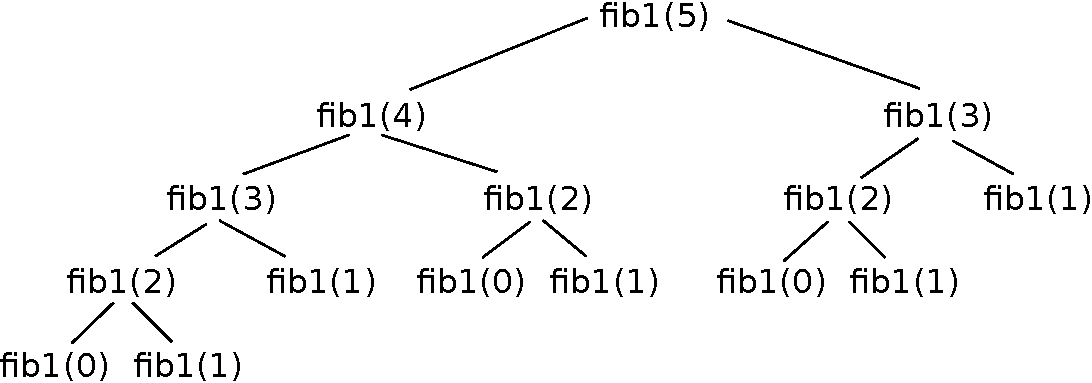
\includegraphics[width = 0.95\linewidth]{./images/fib.pdf}
	\end{figure}
\end{frame}

\begin{frame}[fragile]{Exemple: la suite de Fibonacci}
\textbf{Opération élémentaire} = addition ($+$).\\
La complexité se mesure ici en nombre d'additions (\textit{i.e.} en nombre d'appels à la fonction).
\begin{itemize}
\item \texttt{fibonacci(0)}: $0$
\item \texttt{fibonacci(1)}: $0$
\item \texttt{fibonacci(2)}: $1$
\item \texttt{fibonacci(3)}: $2$
\item \texttt{fibonacci(4)}: $4$
\item \texttt{fibonacci(5)}: $7$
\item \texttt{fibonacci(6)}: $12$
\item \texttt{fibonacci(12)}: $20$
\end{itemize}
\end{frame}

\begin{frame}{Exemple: la suite de Fibonacci}
Si $A_n$ représente le nombre d'additions à faire au rang $n$:
\begin{equation*}
\begin{array}{ccccc}
2 \times A_{n-2} & \leq & A_n & \leq & 2 \times A_{n-1}\\
2^{\frac{n}{2}} & \leq & A_n & \leq & 2^{n}
\end{array}
\end{equation*}
Ceci donne une complexité $C_\text{fibonacci}$ telle que:
$$ O(2^{\frac{n}{2}}) \leq C_\text{fibonacci} \leq O(2^n)$$
\begin{alertblock}{En pratique\dots}
Impossible à calculer pour des $n$ grands.
\end{alertblock}
\end{frame}

\begin{frame}[fragile]{Exemple: la suite de Fibonacci}

Une seconde méthode, non récursive:
\begin{minted}{cpp}
int fibonacci(int n){
    // Initialisation des deux premiers termes
    int fn_m2 = 1, fn_m1 = 1 ;
    for(int i=2; i <= n; i++) {
        int fn = fn_m2 + fn_m1
        // Décalage du rang n-1 au rang n
        fn_m2 = fn_m1;
        fn_m1 = fn;
    }
    return fnm1;
}
\end{minted}
\end{frame}

\begin{frame}{Exemple: la suite de Fibonacci}
L'algorithme ainsi réécrit ne comporte qu'une seule boucle constituée uniquement d'opérations en temps constant.

La complexité $C_\text{fibonacci}$ est en $O(n)$.

\begin{alertblock}{Verdict}
  Le choix de l'implémentation d'un même calcul peut beaucoup influer sur la performance.
\end{alertblock}
\begin{exampleblock}{Remarque}
  La récursivité n'est pas une mauvaise chose, elle est utile quand elle \textbf{ne recalcule pas} plusieurs fois la même chose.
\end{exampleblock}
\end{frame}

\section{Complexité minimale}

\begin{frame}
\frametitle{Complexité minimale}
\begin{block}{Théorème}
Soit $L = \{ a_1, a_2, \ldots, a_n\}$ un ensemble de $n$ valeurs dans $E$ un \textbf{ensemble continu} ou de grand cardinal.

La \textbf{complexité minimale} d'un algorithme de tri prenant en entrée $L$ et renvoyant en sortie les valeurs $a_i$ ordonnées par ordre croissant est $\Theta(n \log{n})$ (linéarithmique).
\end{block}
\end{frame}

\begin{frame}
\frametitle{Complexité minimale: preuve}
\begin{block}{Propriétés d'un algorithme de tri}
\begin{enumerate}
\item Tout algorithme de tri peut se ramener à une succession de comparaisons et de transpositions d'éléments,
	\begin{itemize}
		\item l'opération élémentaire pour la complexité en temps sera la comparaison entre deux éléments du tableau.
	\end{itemize}
\item Tout algorithme de tri doit être capable de trier n'importe quelle liste arbitraire, c'est-à-dire de trier les $n!$ permutations possibles de n'importe quelle liste.
\end{enumerate}
\end{block}
\end{frame}

\begin{frame}{Complexité minimale: preuve - Arbre de tri}
\begin{block}{Lemme}
  On peut représenter un algorithme de tri sous la forme d'un arbre:
  \begin{itemize}
	\item chaque nœud correspond à une comparaison,
	\item chaque nœud a deux arêtes, une pour chaque résultat de la comparaison,
	\item chaque feuille est une permutation possible de la liste d'entrée.
  \end{itemize}
\end{block}
\begin{block}{Conséquences}
  \begin{itemize}
  \item L'arbre est un arbre binaire de hauteur $h$ à $2^h$ feuilles.
  \item L'arbre a au minimum $n!$ feuilles.
  \item La hauteur de l'arbre est le nombre de comparaisons nécessaires pour obtenir une liste triée.
  \end{itemize}
\end{block}
\end{frame}

\begin{frame}{Complexité minimale: preuve - Arbre de tri - Exemple}
  Exemple pour $n=3$ et pour le tri à bulles: \textbf{abc}.
  \begin{figure}
    \centering
    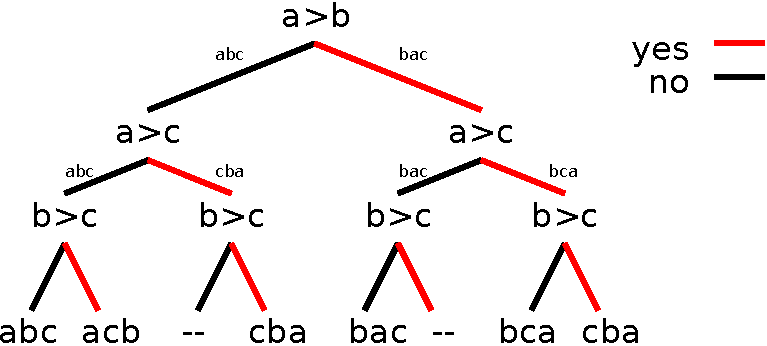
\includegraphics[width = 0.95 \linewidth]{./images/arbreTri.pdf}
  \end{figure}
\end{frame}

\begin{frame}{Complexité minimale des tris (1/2)}
  Chaque feuille de l'arbre est:
  \begin{itemize}
      \item soit vide car correspond à un ordonnancement impossible,
      \item soit une des permutations possibles de la liste.
  \end{itemize}

  Par conséquent, le nombre de feuilles de l'arbre est \textbf{supérieur} au nombre de permutations de la liste d'entrée
  $$n! \leq 2^h$$

  ce qui implique $\log_2 (n!) \leq h.$

  \uncover<2>{En utilisant la formule de Stirling, $ n! \sim \sqrt{2 \pi n}\left( \frac{n}{e}\right)^n$, il vient
	$$h \geq n \cdot \log_2(n) - \frac{n}{\ln 2} = \Theta(n \cdot \log_2 n)$$
  }
\end{frame}

\begin{frame}{Complexité minimale des tris (2/2)}
	D'une part, nous venons de montrer que
	$$h \geq \Theta(n \cdot \log_2 n)~~.$$

	D'autre part, il existe des algorithmes de tri de complexité $\Theta(n\log n)$ donc $h \geq \Theta(n \cdot \log n)$.

	Finalement, il vient:
	$$\boxed{h = \Theta(n \log n).}$$

	$h$ étant la hauteur de l'arbre mais aussi le nombre de comparaisons entre éléments de la liste.
\end{frame}


\begin{frame}[fragile]{Complexité minimale: exemple}
  Exemple du calcul de l'histogramme d'une image.
 \begin{minted}{cpp}
int histo[256];
for(int i=0; i < 256; i++){
    histo[i] = 0;
}
for(int x=0; x < image.width(); x++){
    for(int y=0; y < image.height(); y++){
        histo[image(x,y)]++;
    }
}
\end{minted}
\uncover<2->{
	Chaque pixel doit être observé au moins une fois: $O(n)$.\\
	La complexité minimale n'est pas liée à l'implémentation mais à la tâche à effectuer.
}
\end{frame}

\begin{frame}{Remarque à méditer}

Le théorème de la complexité minimale des algorithmes de tri n'est valable que pour des tableaux à valeurs dans de grands ensembles (de cardinal infini ou presque).

\begin{exampleblock}{Exercice}
	\begin{itemize}
		\item Proposer un algorithme de tri en $O(n)$ pour un tableau de $n$ éléments à valeurs entières dans $\llbracket 0, k\rrbracket$.
	\end{itemize}
\end{exampleblock}

\end{frame}

\section{Algorithmes quadratiques}

\begin{frame}[fragile]{Le tri à bulles}
  \begin{minted}{cpp}
    for(int i=n; i > 0; i--){
      for(int j=0; j < i-1; j++){
        if(t[j] > t[j+1]){
          swap(t[j], j[j+1])
        }
      }
    }
  \end{minted}
  \begin{block}{Complexité}
    Le tri à bulles réalise $(n-1) + (n-2) + \hdots + 1  = \frac{(n-1)(n-2)}{2}$ comparaisons.

    La complexité du tri à bulles est en $O(n^2)$ en moyenne et dans le pire des cas.
  \end{block}
  
  \begin{exampleblock}{Autres algorithmes classiques en $O(n^2)$}
  Le tri par insertion et le tri par sélection sont de complexité quadratique.
  \end{exampleblock}
\end{frame}

\section{\emph{QuickSort}: le tri rapide}

\begin{frame}{QuickSort: principe}
  \begin{enumerate}
      \item Choisir un élément du tableau, il devient \textbf{le pivot}.
      \item Placer le pivot à la position $i$ de sorte que tous les éléments d'indice inférieurs à $i$ soient plus petits que le pivot et tous les éléments d'indice supérieurs à $i$ soient plus grands.
      \item Réitérer le procédé sur chacune des deux sous-parties du tableau.
  \end{enumerate}
\end{frame}

\begin{frame}{QuickSort: placer le pivot}
\begin{figure}
\centering
\includegraphics<1>[width = 0.95\linewidth]{./images/quick1.pdf}
\includegraphics<2>[width = 0.95\linewidth]{./images/quick2.pdf}
\includegraphics<3>[width = 0.95\linewidth]{./images/quick3.pdf}
\includegraphics<4>[width = 0.95\linewidth]{./images/quick4.pdf}
\includegraphics<5>[width = 0.95\linewidth]{./images/quick5.pdf}
\includegraphics<6>[width = 0.95\linewidth]{./images/quick6.pdf}
\includegraphics<7>[width = 0.95\linewidth]{./images/quick7.pdf}
\includegraphics<8>[width = 0.95\linewidth]{./images/quick8.pdf}
\includegraphics<9>[width = 0.95\linewidth]{./images/quick9.pdf}
\includegraphics<10>[width = 0.95\linewidth]{./images/quick10.pdf}
\includegraphics<11>[width = 0.95\linewidth]{./images/quick11.pdf}
\includegraphics<12>[width = 0.95\linewidth]{./images/quick12.pdf}
\includegraphics<13>[width = 0.95\linewidth]{./images/quick13.pdf}
\includegraphics<14>[width = 0.95\linewidth]{./images/quick14.pdf}
\includegraphics<15>[width = 0.95\linewidth]{./images/quick15.pdf}
\includegraphics<16>[width = 0.95\linewidth]{./images/quick16.pdf}
\includegraphics<17>[width = 0.95\linewidth]{./images/quick17.pdf}
\includegraphics<18>[width = 0.95\linewidth]{./images/quick18.pdf}
\includegraphics<19>[width = 0.95\linewidth]{./images/quick19.pdf}
\includegraphics<20>[width = 0.95\linewidth]{./images/quick20.pdf}
\end{figure}
\end{frame}

\begin{frame}{Complexité de Quicksort}

\begin{block}{Théorème}
Quicksort est un tri en $O(n\log(n))$ \textbf{en moyenne}.
\end{block}

\vspace{1cm}
\textit{Démonstration dans le chapitre 3.}

\end{frame}


\begin{frame}{QuickSort: complexité - Pire des cas}

Le parcours du tableau implique $n-1$ comparaison. Donc:
$$ C_n = (n-1) + C_i + C_{n-i-1}$$
Si on suppose que $i = n-1$ (déjà triée):
$$ C_n = (n-1) + C_{n-2}$$
Au rang suivant:
$$ C_n = (n-1) + (n-2)+ C_{n-3}$$

En fait, cela revient à effectuer un tri à bulles:
$$C_n = O(n^2)$$
\end{frame}

\begin{frame}{QuickSort: éviter le pire des cas}
Pour éviter le pire des cas en moyenne on utilise généralement:
\begin{itemize}
\item un tirage du pivot au hasard
\item un pivot au milieu du tableau
\item un mélange de la liste au préalable
\end{itemize}
\end{frame}

\begin{frame}{QuickSort: en pratique}

\begin{itemize}
\item QuickSort est implémenté dans la STL (\texttt{\#include <algorithm>}).
\item Il existe des algorithmes en $O(n \log{n})$ quoi qu'il arrive (tri par tas, tri fusion, \dots), mais il sont moins rapides que QuickSort \textbf{en moyenne}.
\end{itemize}

\end{frame}

\section{Tri par tas}

\begin{frame}{File de priorité}

La file de priorité est une structure de données permettant~:
\begin{itemize}
\item Accès à l'élément le plus prioritaire en $O(1)$
\item Ajout d'un élément en $O(\log n)$
\item Retrait d'un élément en $O(\log n)$
\end{itemize}

\vspace{1cm}
\textit{Étude de la file de priorité au chapitre 4.}
\end{frame}

\begin{frame}[fragile]{Tri par tas}

Le tri par tas remplit une file de priorité et puis retire les éléments un par un.
\begin{minted}{cpp}
void HeapSort(std::vector<double> &v){
  FilePriorite f;
  for(int i=0; i < v.size(); i++){
    f.push(v[i]);
  }
  for(int i=0; i < v.size(); i++){
    v[i] = f.pop();
  }
}
\end{minted}
\end{frame}

\begin{frame}{Conclusion}
Le tri par tas est un tri en $O(n \log n)$ dans tous les cas. Cependant en comparaison à QuickSort, il utilise plus de mémoire et est plus long en moyenne.

En pratique c'est QuickSort le plus utilisé.
\end{frame}


\begin{frame}{Tri par tas: complexités à retenir}

\begin{itemize}
\item Tri: $O(n \log n)$
\item Recherche dans un tableau trié: $O(\log n)$
\item Recherche dans un tableau non trié: $O(n)$
\end{itemize}

\end{frame}

\section{Recherche dans un tableau}

\begin{frame}{Recherche dans un tableau non trié}

\begin{block}{Tableau non trié}
Pas d'a priori sur la structure du tableau. Il faut regarder chaque élément.
\end{block}

\begin{block}{Complexité}
$$O(n)$$
\end{block}

\end{frame}

\begin{frame}[fragile]{Recherche dichotomique}

Le fait de savoir que le tableau est trié permet de réduire la complexité de la recherche à $O(\log(n))$.

\begin{minted}{cpp}
int dichotomie(const std::vector<double>& V, double val){
    int debut = 0, fin = v.size() - 1;
    while(debut < fin){
        int milieu = (debut + fin)/2;
        if(V[milieu] == val)
            return milieu;
        if(V[milieu] < val){
            debut = milieu + 1;
        } else {
            fin = milieu - 1;
        }
    }
    // On renvoie l'indice actuel si c'est la bonne valeur
    // ou -1 sinon car la valeur n'est pas dans le vecteur
    return (V[milieu] == val) ? a:-1;
}
\end{minted}
\end{frame}

\begin{frame}{Codons!}

\begin{block}{Travaux pratiques}
	Implémentation de quelques algorithmes de tri en C++.
\end{block}

\begin{alertblock}{Exercices bonus}
Pour voir des problèmes un peu différents\dots
\end{alertblock}
\end{frame}

\end{document}
